\documentclass[10pt,a4paper]{cerndoc}

\CernDocSection{CERN BE-CO-HT}
\CernDocBorderColor{10,120,10}

\CernDocType{Functional Specifications}
\CernDocTitle{Gennum GN4124 Core For FMC Projects}
\CernDocEditedBy{Simon Deprez}
\CernDocCheckedBy{Javier Serrano}
\CernDocDate{July 2010}
\CernDocAbstract{This functional specification describes the HDL controller for Gennum the GN4124 chip. This chip is used on the PCI express FMC carrier (\href{http://www.ohwr.org/projects/fmc-pci-carrier}{www.ohwr.org/projects/fmc-pci-carrier}). It provides a Wishbone master for control and status registers access and a DMA controller for high speed data transfers.}

\widowpenalty 10000
\clubpenalty 10000
\raggedbottom

\begin{document}
  \cerntitle
  \section*{Revision History}
  \begin{tabularx}{\textwidth}{|p{3cm}|p{3cm}|X|}
    \hline \textbf{Version}&\textbf{Date}&\textbf{Notes}\\ \hline \hline
    0.1 & 21-05-2010 & Initial release\\ \hline
    0.2 & 29-05-2010 & Add DMA master specifications\\ \hline
    0.3 & 01-06-2010 & Core diagram review + clocks\\ \hline
    0.4 & 28-06-2010 & Add byte swapping for DMA interface\\ \hline
    0.5 & 06-07-2010 & Corrections after review of 25-06-10\\ \hline

  \end{tabularx}

  \tableofcontents
  \listoffigures
  \listoftables
  \clearpage

%  \section*{Introduction}
%  \addcontentsline{toc}{section}{Introduction}

  \section{Introduction}
The PCIe FMC carrier\footnote{See \href{http://www.ohwr.org/projects/fmc-pci-carrier}{www.ohwr.org/projects/fmc-pci-carrier}.} will be associated with several FMC\footnote{See VITA FMC standard: \href{http://www.vita.com/fmc}{www.vita.com/fmc}.} mezzanines. 

Each FMC mezzanine used with the PCIe FMC carrier will need a specific HDL (Hardware description language) configuration. The HDL code should be generic for reusing the carrier-specific modules with the other FMC mezzanines. 

 The communication between modules is essentially based on the Wishbone bus. Two separates Wishbones bus are used to performs communications.
 
\begin{packed_item}
  \item CSR (Control and status register) Interface 
  %\item 1 Wishbone master interface that transforms memory reads and memory writes from PCI express bus in Wishbone single reads and single writes. (20 MB/s -- 100 MB/s)
  \begin{packed_item}
    \item Wishbone\footnote{See \href{http://opencores.org/opencores,wishbone}{http://opencores.org/opencores,wishbone}.} Master
  	\item 32 bit  
  	\item Singles reads and writes 
  	\item 40 MB/s (single reads) -- 200 MB/s (single writes)
   \end{packed_item}  
  
  \item DMA Interface 
%\item 1 DMA master interface that preforms data transfers from local application to PCI express host. (up to 400 MB/s)
  \begin{packed_item}
    \item Pipelined Wishbone Master
  	\item 32 bit  
  	\item Local to PCI Express data transfer
  	\item PCI Express to local data transfer
  	\item Byte swapping
  	\item 600 MB/s 
   \end{packed_item}     
   


\end{packed_item}

  \section{GN4124 core for PCIe FMC carrier}
  This core provides a Wishbone master to access control registers and read status.  The Wishbone bus is used for almost all communications between modules. The different soft cores are reusable.
  
  A simple DMA master is used for high speed data transfers of mezzanine card acquisitions. This DMA master is also based on Wishbone and uses a new pipelined mode that was developed to increase  throughput.
  
\begin{figure}[!ht]
	\centering
		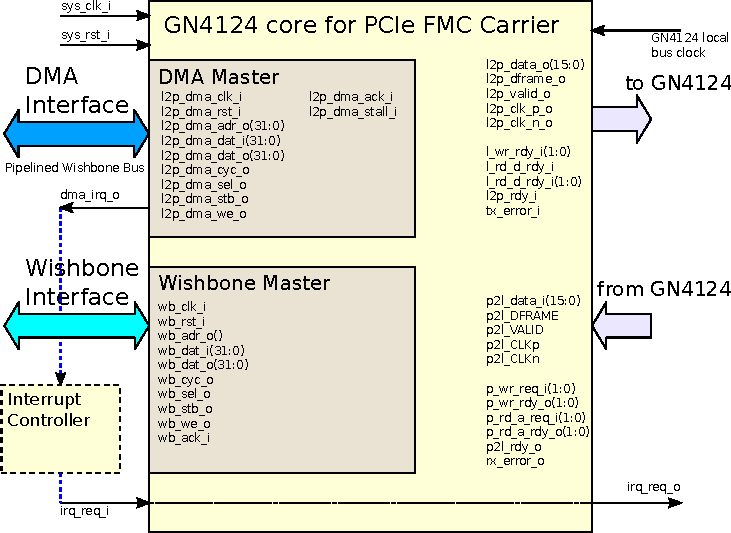
\includegraphics[width=\textwidth]{GN4124core.pdf}
	\caption{GN4124 core for PCIe FMC carrier}
	\label{fig:GN4124core}
\end{figure} 
    \subsection{GN4124 Local Bus Interface}
    
The GN4124 is a 4-lane PCI express to local bus bridge that is designed to work with an FPGA device to provide a high speed serial access for an application.
    
The GN412x PCI Express family Reference Manual\footnote{See \href{http://my.gennum.com/mygennum/view.php/gn4124-gullwing}{http://my.gennum.com/mygennum/view.php/gn4124-gullwing}.} (52624-0 June 2009) describes the local bus interface at page 40.

The data exchange is based on packets similar to PCI express packets, but the headers are different. It is not possible to send MSI (Message Signaled Interrupts) packets with this bus so the interrupt request signal is wired to a GPIO input of the GN4124 chip.
    
    \subsection{DMA Interface}
The DMA interface is a 32 bit pipelined Wishbone bus. It preforms data transfers from local application to PCI express host.

The DMA engine works with a linked list so that DMAs can be chained. The first item in the list is loaded by the host on the carrier and contains a pointer to the next one, which is in host memory. The DMA engine will fetch items from host memory and perform the corresponding DMAs until one of the items is recognized as the last one though the contents of the DMAATTRIBR register (see table~\ref{tab:dma_control}). 

Each item in the list is made of the following registers: DMACSTARTR, DMAHSTARTLR, DMAHSTARTHR, DMALENR, DMANEXTLR, DMANEXTHR and DMAATTRIBR. When reading these items from the host, the DMA engine assumes a little-endian host. Big-endian hosts should shuffle data accordingly so that it is found in the same order as in a little-endian host. In addition, the DMA controller provides global DMA control and status registers.

The end of a chained DMA access generates an interrupt request (\verb+dma_irq_p1_o+ output) towards the interrupt controller.  

\begin{table}[htbp]
  \centering
  \begin{tabularx}{\textwidth}{|l|c|l|c|X|}                                                   \hline
    \textbf{NAME}  & \textbf{OFFSET} & \textbf{MODE} & \textbf{RESET} & \textbf{DESCRIPTION}  \\ \hline \hline
    DMACTRLR       & 0x00 & R/W & 0x00000000 & DMA engine control                                       \\ \hline
    DMASTATR       & 0x04 & RO  & 0x00000000 & DMA engine status                                              \\ \hline
    DMACSTARTR     & 0x08 & R/W & 0x00000000 & DMA start address in the carrier                               \\ \hline
    DMAHSTARTLR    & 0x0C & R/W & 0x00000000 & DMA start address (low) in the PCIe host                       \\ \hline
    DMAHSTARTHR    & 0x10 & R/W & 0x00000000 & DMA start address (high) in the PCIe host                      \\ \hline
    DMALENR        & 0x14 & R/W & 0x00000000 & DMA read length in bytes                                       \\ \hline
    DMANEXTLR      & 0x18 & R/W & 0x00000000 & Pointer (low) to next item in list                             \\ \hline
    DMANEXTHR      & 0x1C & R/W & 0x00000000 & Pointer (high) to next item in list                            \\ \hline
    DMAATTRIBR     & 0x20 & R/W & 0x00000000 & DMA chain control                                              \\ \hline
  \end{tabularx}
  \caption{Register set for the DMA controller block}
  \label{tab:dma_control}
\end{table}


\newpage
\subsubsection{DMACTRLR}
%Writing 1 to this register starts a DMA transfer. Writing 2 aborts the ongoing transfer.
\begin{packed_item}
\item Bits [31..4] are reserved.
\item Bits [3..2] controls byte swapping of the DMA interface(see table~\ref{tab:byte_swapping}). It works in the both DMA transfer directions:
  \begin{packed_item}
    \item "00" To swapping.
    \item "X1" Swap the two bytes in the words.
    \item "1X" Swap the two words.
  \end{packed_item}
\item Bit 1 is set to '1' to abort the ongoing transfer.
\item Bit 0 is set to '1' to start a DMA transfer, '0' otherwise.
\end{packed_item}

\begin{table}[htbp]
  \centering
  \begin{tabular}{|c|c|c|}                                                      \hline
    Double word on PCI Express & Control bits of the swapping & Double word on Wishbone bus           \\ \hline \hline
     \multirow{4}{*}{A1 B2 C3 D4}
                         &  "00"         &  A1 B2 C3 D4                         \\ \cline{2-3}
                         &  "01"         &  B2 A1 D4 C3                         \\ \cline{2-3}
                         &  "10"         &  C3 D4 A1 B2                         \\ \cline{2-3}
                         &  "11"         &  D4 C3 B2 A1                         \\ \hline

  \end{tabular}
  \caption{Byte swapping}
  \label{tab:byte_swapping}
\end{table}

\subsubsection{DMASTATR}
This is a status register for the DMA engine. Possible contents are:
\begin{packed_item}
\item 0: Idle (before any DMA transfer takes place and after reset).
\item 1: Done (after successful DMA).
\item 2: Busy.
\item 3: Error (following a memory access error, either on the host or on the carrier). This also produces an interrupt.
\item 4: Aborted (after receiving an abort command in DMACTRLR).
\end{packed_item}
A DMA start command written into the DMACTRLR register takes this status out of Idle, Done, Error or Aborted into the Busy state.

\subsubsection{DMACSTARTR}
The DMACSTARTR register holds a byte address pointing to a location inside the local memory, at which the DMA access should start.

\subsubsection{DMAHSTARTLR and DMAHSTARTHR}
Registers DMAHSTARTLR and DMAHSTARTHR select the low and high parts of the 64-bit start address for the DMA access in the PCI Express host. 

\subsubsection{DMALENR}
Register DMALENR selects the length of the data transfer in bytes. 

\subsubsection{DMANEXTLR and DMANEXTHR}
These two registers contain the low and high parts of the 64-bit address of the next item in the linked list, in PCI Express host memory.

\subsubsection{DMAATTRIBR}
This register contains several control features for the DMA engine:
\begin{packed_item}
\item Bits [31..2] are reserved.
\item Bit 1: Transfer direction. This bit is set to '0' for local to PCI Express host data transfer an '1' for PCI Express host to local data transfer.
\item Bit 0 is set to '1' to signal this is the last item in the linked list, '0' otherwise.
\end{packed_item}

The end of a chained DMA access generates an interrupt request towards the interrupt controller.    
    \subsection{Wishbone interface}
    The Wishbone master (see table~\ref{tab:wb_control}) transforms a PCIe memory write into a 32 bits Wishbone write and a PCIe memory read into a 32 bits Wishbone read. Only single reads and writes are supported.   
    
    The Wishbone bus is clocked by the \verb+wb_clk_i+ input.
    
    

\begin{table}[htbp]
  \centering    
    \begin{tabularx}{\textwidth}{|X|cc|} \hline
      \multicolumn{3}{|c|}{WISHBONE DATASHEET for the 32-bit MASTER}                                           \\ \hline \hline
      \multicolumn{1}{|c|}{Description}  &\multicolumn{2}{c|} { Specification}                                 \\ \hline
      General description                &\multicolumn{2}{l|} { Wishbone master controlled by PCI express}     \\ \hline
      Supported cycles                   &\multicolumn{2}{l|} { MASTER, READ/WRITE }                           \\ \hline
      Data port, size:                   &\multicolumn{2}{l|} { 32-bit}                                        \\
      Data port, maximum operand size    &\multicolumn{2}{l|} { 32-bit}                                        \\
      Clock frequency constraints:       &\multicolumn{2}{l|} { 100 MHz}                                       \\ \hline
      \multirow{8}{6cm}{Supported signal list and cross reference to equivalent WISHBONE signals}
      &  Signal Name       & WISHBONE Equiv.                                                                   \\
      &  sys\_clk\_i       &  CLK\_I                                                                           \\
      &  sys\_rst\_i       &  RST\_I                                                                           \\
      &  wb\_cyc\_o        &  CYC\_O                                                                           \\
      &  wb\_stb\_o        &  STB\_O                                                                           \\
      &  wb\_adr\_o(10..0) &  ADR\_O()                                                                         \\
      &  wb\_dat\_i(31..0) &  DAT\_I()                                                                         \\
      &  wb\_dat\_o(31..0) &  DAT\_O()                                                                         \\
      &  wb\_we\_o         &  WE\_O                                                                            \\
      &  wb\_ack\_i        &  ACK\_I                                                                           \\ \hline
	\end{tabularx}
	\caption{Wishbone master datasheet}
  \label{tab:wb_control}
\end{table}

   \subsection{Interrupts}
   When the GN4124 master gets a one-tick-long (\verb+sys_clk_i+) positive pulse on the \verb+irq_req_p1_i+ input, a one-tick-long (GN4124 local bus clock) positive pulse is sent on the \verb+irq_req_p1_o+ output to the GN4124 chip. The interrupt signal is directly wired to GN4124 chip GPIO. When configured, the chip sends an MSI packet (Message Signaled Interrupts) to the host.
   
   At the end of a chained DMA acces, the DMA master sends a one-tick-long (\verb+sys_clk_i+) interrupt signal on the \verb+dma_irq_p1_o+ output toward the interrupt controller (see figure~\ref{fig:GN4124core}). So the interrupt controller knows that the DMA master is the source of the interrupt.

\end{document}







